\section{Implementation Details for Crystal Plasticity}\label{app:cp3d_details}

{This appendix specifies the local constitutive equations, data-generation procedure, and training setup for the crystal-plasticity experiments in Section~\ref{subsec:3d_crystal_plasticity}.}

{\color{blue}
\subsection{Constitutive Equations}\label{app:cp3d_constitutive}
The cell problem \cref{eq:cp_cell_problem} is closed by the following local constitutive equations. We use the multiplicative decomposition into elastic and plastic distortions, $F=F_eF_p$, with elastic Green--Lagrange strain and stress
\begin{align*}
    E_e&=\tfrac12(F_e^{\top}F_e-I),
    &S_e&=\bC_{\rm crys}E_e,
    &P&=F_eS_eF_p^{-\top}.
\end{align*}
Here $\bC_{\rm crys}$ is the cubic single-crystal stiffness and $S_e$ is the elastic second Piola--Kirchhoff stress. The stiffness and slip systems are expressed in crystal coordinates. Plastic flow on the twelve FCC $\{111\}\langle110\rangle$ systems satisfies
\begin{align*}
    \dot F_p=L_pF_p,\qquad L_p=\sum_{\alpha=1}^{12}\dot\gamma^\alpha s^\alpha\otimes m^\alpha,\qquad \dot\gamma^\alpha=\dot\gamma_0\left|\frac{\tau^\alpha}{r^\alpha}\right|^n\operatorname{sgn}(\tau^\alpha),\qquad \tau^\alpha=S_e(s^\alpha\otimes m^\alpha),
\end{align*}
where $\dot\gamma^\alpha$ is the shear rate on system $\alpha$, with unit slip direction $s^\alpha$, unit plane normal $m^\alpha$, and slip resistance $r^\alpha$. The resolved shear stress follows DAMASK's small-elastic-strain approximation $F_e^{\top}F_e\simeq I$ in the plastic driving stress \cite[Appendix C]{roters2019damask}. The slip resistances evolve by self and latent hardening according to
\begin{equation*}
    \dot r^\alpha=h_0\operatorname{sgn}\!\left(1-\frac{r^\alpha}{r_\infty}\right)\left|1-\frac{r^\alpha}{r_\infty}\right|^a\sum_{\beta=1}^{12}Q_{\alpha\beta}|\dot\gamma^\beta|.
\end{equation*}
Here $h_0(y)$ is the hardening scale, $r_\infty(y)$ is the saturation resistance, and $Q_{\alpha\beta}$ is the FCC slip-interaction matrix. The initial orientation $O_0(y)$ maps specimen coordinates to crystal coordinates and is incorporated into the initial plastic distortion. With initial slip resistance $r_0(y)$, the initially stress-free state is specified by
\begin{equation*}
    \chi(y,0)=0,\qquad F_p(y,0)=O_0(y),\qquad r^\alpha(y,0)=r_0(y).
\end{equation*}
Since $\overline F(0)=I$, these conditions give $F_e(y,0)=O_0(y)^{\top}$ and $S_e(y,0)=0$.

The elastic constants are $(C_{11},C_{12},C_{44})=(168.9,121.8,75.8)\,\mathrm{GPa}$, the reference shear rate is $\dot\gamma_0=3\times10^{-3}\,\mathrm{s}^{-1}$, the rate exponent is $n=20$, and the saturation exponent is $a=0.6$. The seven coefficients defining $Q$ are $(1,1,5.123,0.574,1.123,1.123,1)$ for self, coplanar, collinear, Hirth, glissile I, glissile II, and Lomer interactions, respectively.} The grainwise fields $r_0$, $r_\infty$, and $h_0$ are sampled as follows.


\subsection{Microstructure Sampling}\label{app:cp3d_microstructure_sampling}
{Let $\{G_j\}_{j=1}^{N_g}$ denote the grains of the periodic Voronoi tessellation. The microstructural input is piecewise constant on grains, with $M(y)=(q_j,r_{0,j},r_{\infty,j},h_{0,j})\in\bR^7$ for $y\in G_j$. Here $q_j\in\bR^4$ is the orientation quaternion representing $O_0$ on $G_j$. For the single- and two-mode textures, the spread angle is sampled over the range $5^{\circ}$ to $35^{\circ}$.}

{
We sample the three slip-law parameters around the copper reference values using correlated grainwise scale factors. For each sample, we draw $\delta\sim\mathrm{Unif}[0.05,0.20]$, a resistance scale $\bar s_r$ log-uniformly from $[0.80,1.35]$, and a hardening scale $\bar s_h$ log-uniformly from $[0.80,1.50]$. For each grain $G_j$, we draw a standard Gaussian pair $(Z_{r,j},Z_{h,j})$ with correlation $0.65$ and set
\begin{equation*}
    s_{r,j}=\bar s_r\exp(\delta Z_{r,j}),\qquad s_{h,j}=\bar s_h\exp(\delta Z_{h,j}).
\end{equation*}
We set
\begin{equation*}
    r_{0,j}=31\,\mathrm{MPa}\,s_{r,j},\qquad r_{\infty,j}=96.4\,\mathrm{MPa}\,s_{r,j},\qquad h_{0,j}=0.35\,\mathrm{GPa}\,s_{h,j}.
\end{equation*}
Thus $r_{0,j}$ and $r_{\infty,j}$ vary together with a constant ratio, while $h_{0,j}$ varies through a distinct but positively correlated factor.
}

\subsection{Trajectory Sampling}\label{app:cp3d_loading_sampling}
We parameterize each macroscopic loading path by separating the rotation, volumetric stretch, and deviatoric stretch components. Specifically, we write
\begin{equation*}
    \overline F(t)=R(t)\exp(E(t)),
    \quad
    R(t)=\exp(\operatorname{skew}(\omega(t))),
\end{equation*}
where $E(t)$ is the logarithmic strain, $\omega(t)\in\bR^3$ is the rotation vector, and {$\operatorname{skew}(\omega(t))$} is the associated skew symmetric matrix, i.e., $\operatorname{skew}(w)v=w\times v$ for $v,w\in\bR^3$. The logarithmic strain is decomposed as
\begin{equation*}
    E(t)=\frac{\eta_{\rm vol}(t)}{3}I+E_{\rm dev}(t),
    \quad
    \eta_{\rm vol}(t)=\log\det\overline F(t),
    \quad
    \operatorname{tr}E_{\rm dev}(t)=0.
\end{equation*}
After choosing a basis $\{B_a\}_{a=1}^{5}$ for trace-free symmetric $3\times3$ tensors, we have $E_{\rm dev}(t)=\sum_{a=1}^{5}e_a(t)B_a$.
Thus, each loading path is sampled through the nine scalar coordinates $\left(\eta_{\rm vol}(t),e_1(t),\dots,e_5(t), \omega_1(t),\omega_2(t),\omega_3(t)\right)$
independently according to the procedure in \cref{app:kv2d_strain_sampling}. The initial scalar values are set so that $\overline F(0)=I$. Once the scalar paths have been sampled and interpolated, the deformation gradient is reconstructed on the common output time grid. This reconstruction enforces $\det\overline F(t)=\exp(\eta_{\rm vol}(t))>0$.

\subsection{Architecture and Training}\label{app:cp_training}
The architecture and training are similar to \cref{app:kv2d_training}, except that we use 8 Fourier modes, a width of 48, and a projection width of 96. We use a penalty weight of $\alpha=0.001$ across all internal-variable dimensions. We train on trajectory data with a larger step size (1/64) rather than the data-generation step size (1/128), and only on [0, 0.875] rather than the full unit time interval. This reduction lets us make the most of our computing resources; we use 4 Nvidia Tesla P100 GPUs for training. The testing is performed on the full trajectory data.

\subsection{Median-Error Prediction Visualization}

\Cref{fig:cp_median_prediction} shows the median-error test sample for the crystal-plasticity dataset, including the sampled microstructure, loading path, stress response, and learned internal variables.

\begin{figure}[!htp]
    \centering
    {\bf The median error test sample: Crystal plasticity dataset}\\[5pt]
    \scalebox{0.7}{
\addtolength{\tabcolsep}{-5 pt}
    \begin{tabular}{>{\centering\arraybackslash} m{0.18\linewidth} >{\centering\arraybackslash} m{0.06\linewidth}
    >{\centering\arraybackslash} m{0.16\linewidth} 
    >{\centering\arraybackslash} m{0.16\linewidth}
    >{\centering\arraybackslash} m{0.16\linewidth}}
        \raisebox{-40 pt}{\multirow{4}{*}{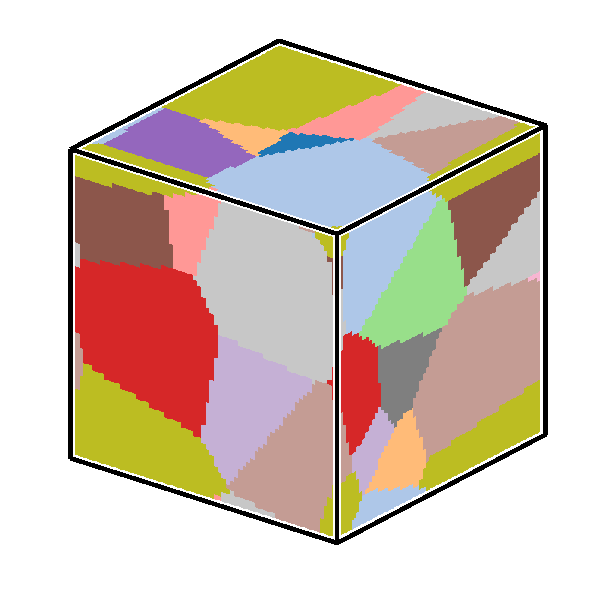
\includegraphics[width=\linewidth]{figures/grain_id_median.pdf}}} & \raisebox{45 pt}{\multirow{2}{*}{\rotatebox[origin=c]{90}{\makecell{Slip-law parameters \\ (MPa)}}}} &
        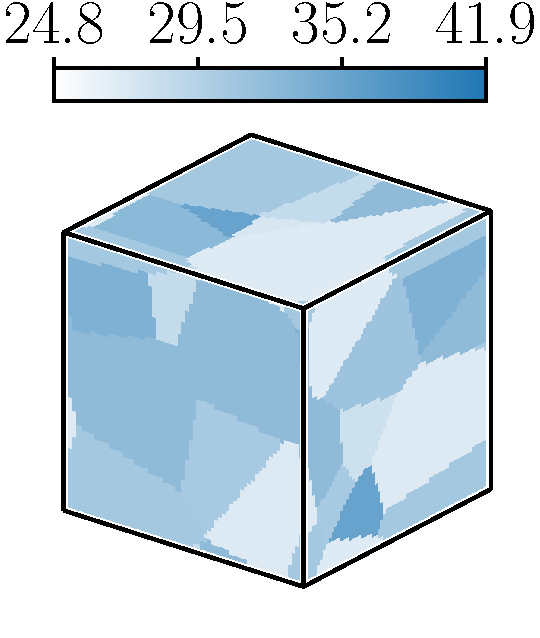
\includegraphics[width=\linewidth]{figures/xi_0_sl_median.pdf}  & 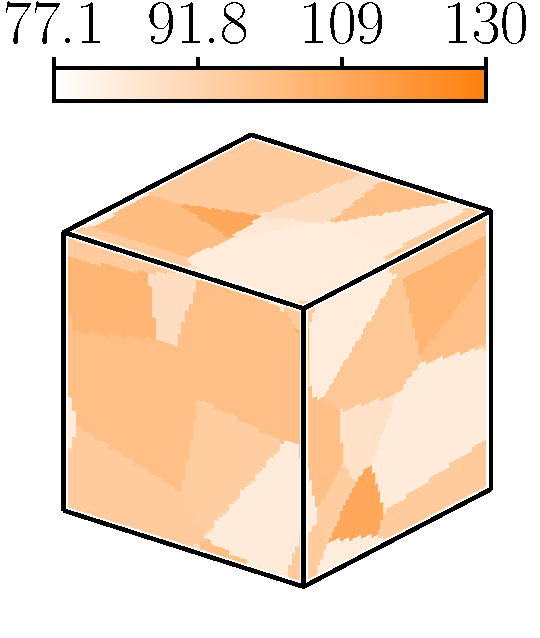
\includegraphics[width=\linewidth]{figures/xi_inf_sl_median.pdf} & 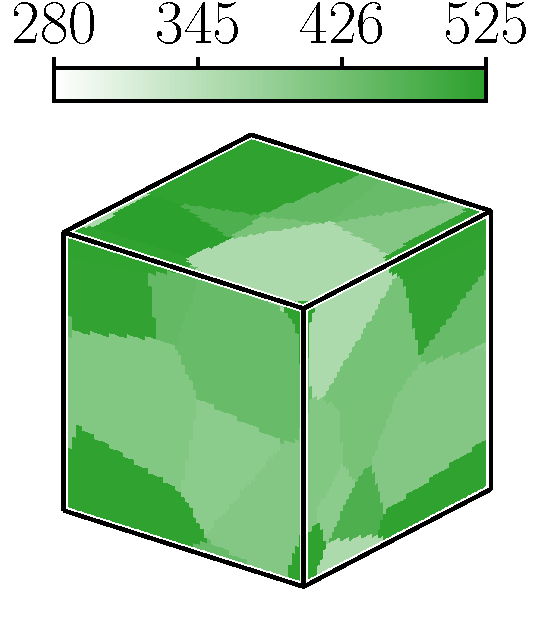
\includegraphics[width=\linewidth]{figures/h_0_sl_median.pdf} \\
         & & Initial slip resistance &Saturation slip resistance & Hardening scale \\
            & \raisebox{40 pt}{\rotatebox[origin=b]{90}{Pole figures}} & \multicolumn{3}{c}{\parbox[c]{0.48\linewidth}{\centering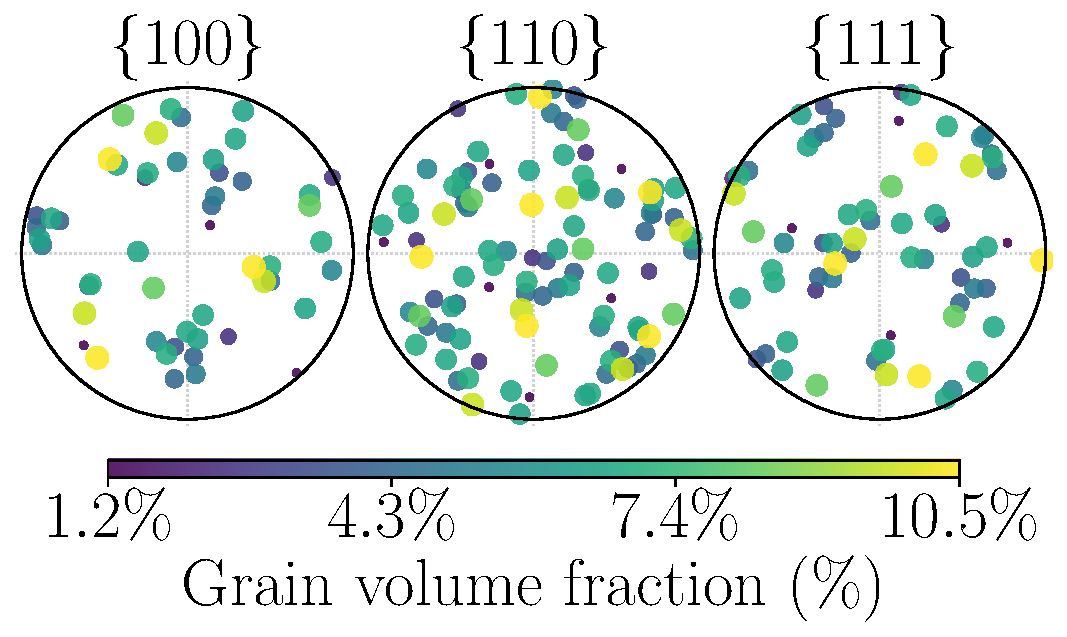
\includegraphics[width=0.875\linewidth]{figures/texture_median.pdf}}}  \\
    \end{tabular}
    \begin{tabular}{c}
         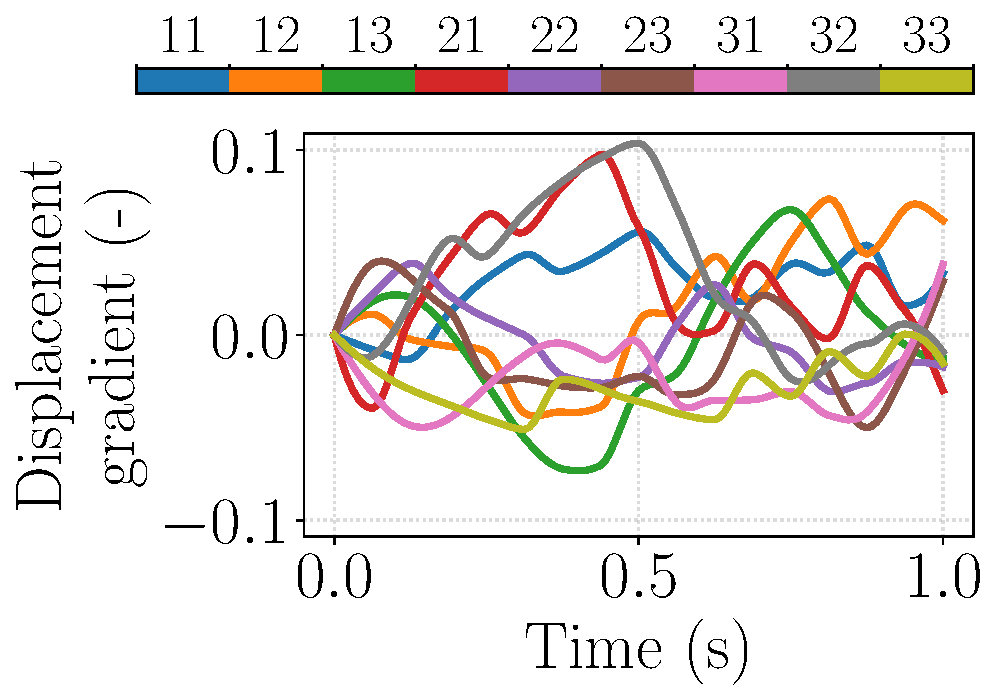
\includegraphics[width=0.4\linewidth, trim={0 1.0in 0 0},clip]{figures/displacement_gradient_median.pdf}  \\
        \hspace{0.012\linewidth}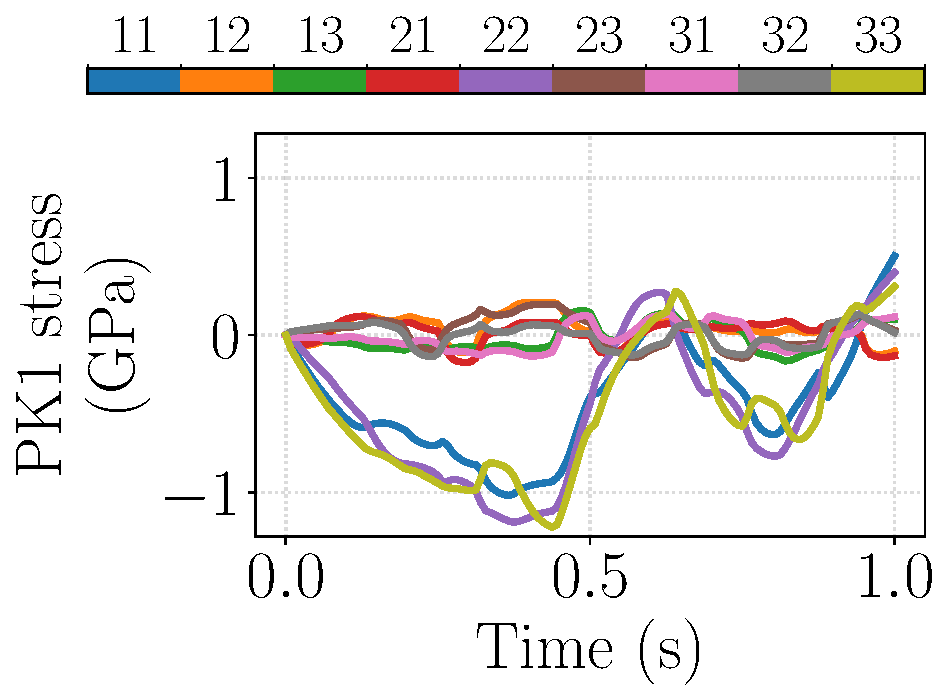
\includegraphics[width=0.39\linewidth, trim={0 0 0 0.8in},clip]{figures/pk1_stress_median.pdf}
    \end{tabular}
\addtolength{\tabcolsep}{5 pt}
    }
\scalebox{0.5}{
\addtolength{\tabcolsep}{-5 pt}
\centering
        
        \begin{tabular}{c c c c}
        & 11 & 12 & 13 \\
        \multirow{3}{*}{\rotatebox[origin=c]{90}{PK1 Stress (GPa)}}&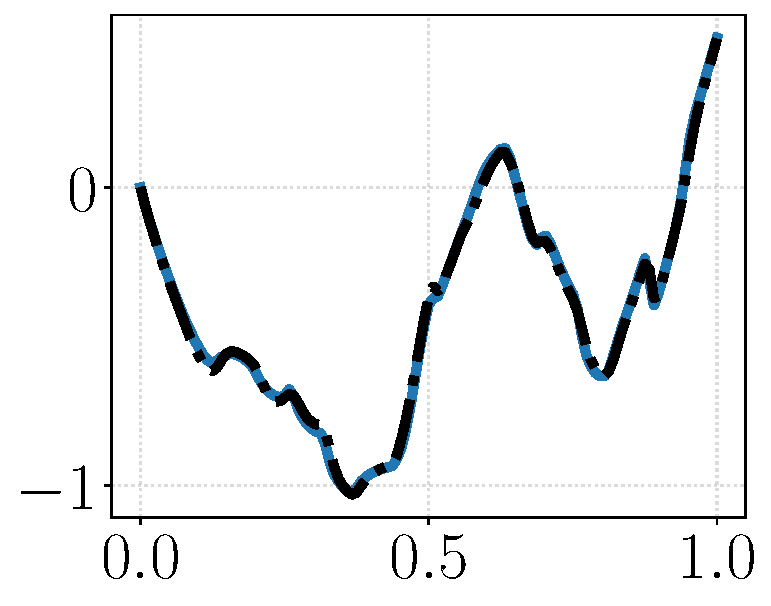
\includegraphics[width=0.25\linewidth]{figures/pk1_stress_11_median.pdf} &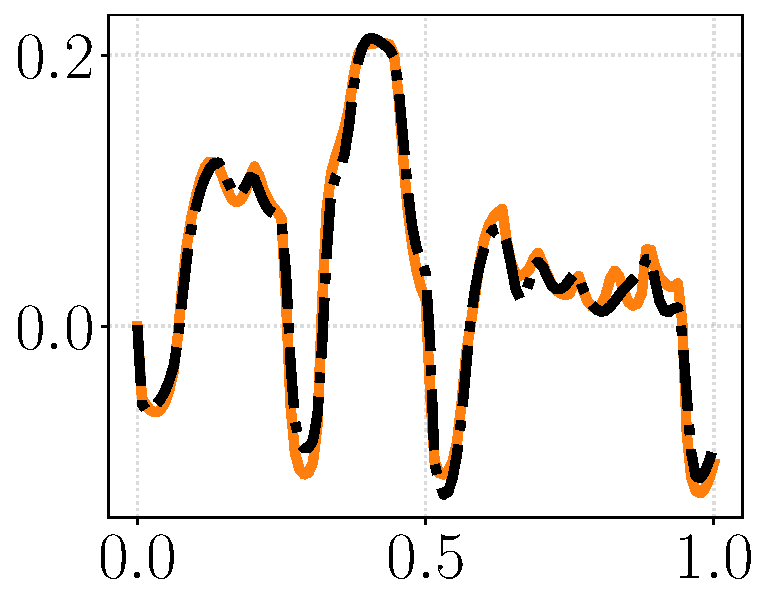
\includegraphics[width=0.25\linewidth]{figures/pk1_stress_12_median.pdf}  
         & 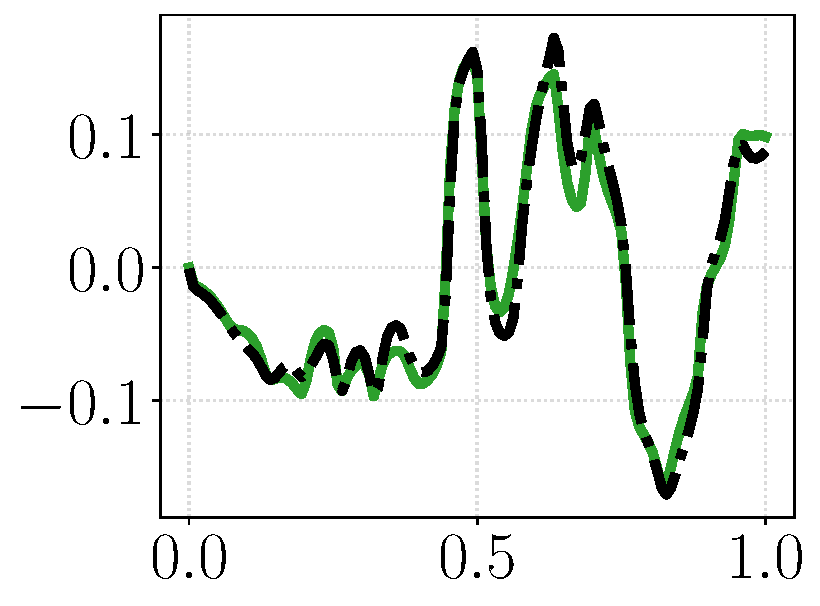
\includegraphics[width=0.265\linewidth]{figures/pk1_stress_13_median.pdf} \\
        & 21 & 22 & 23 \\
         &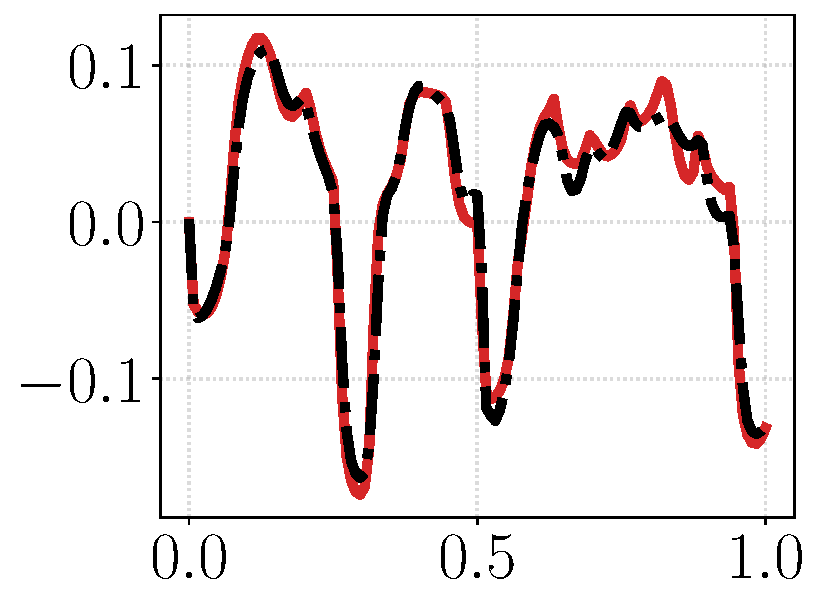
\includegraphics[width=0.26\linewidth]{figures/pk1_stress_21_median.pdf} &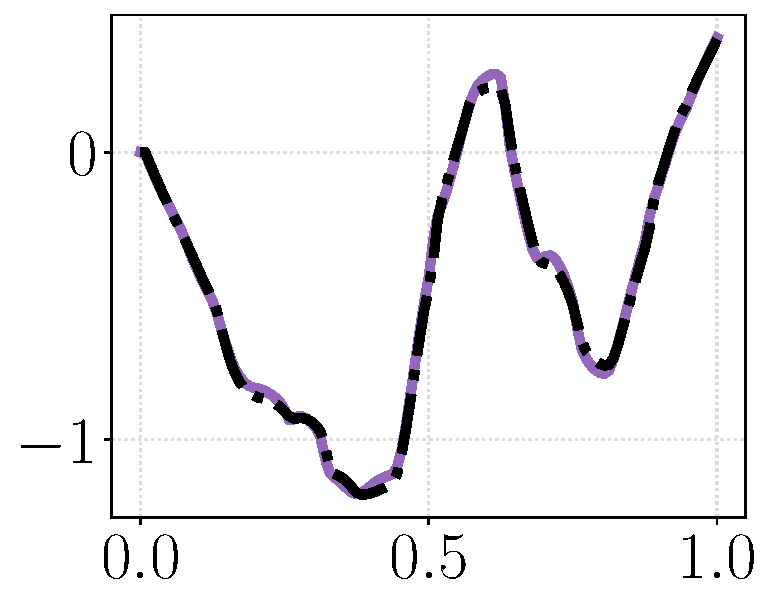
\includegraphics[width=0.245\linewidth]{figures/pk1_stress_22_median.pdf}  
         & 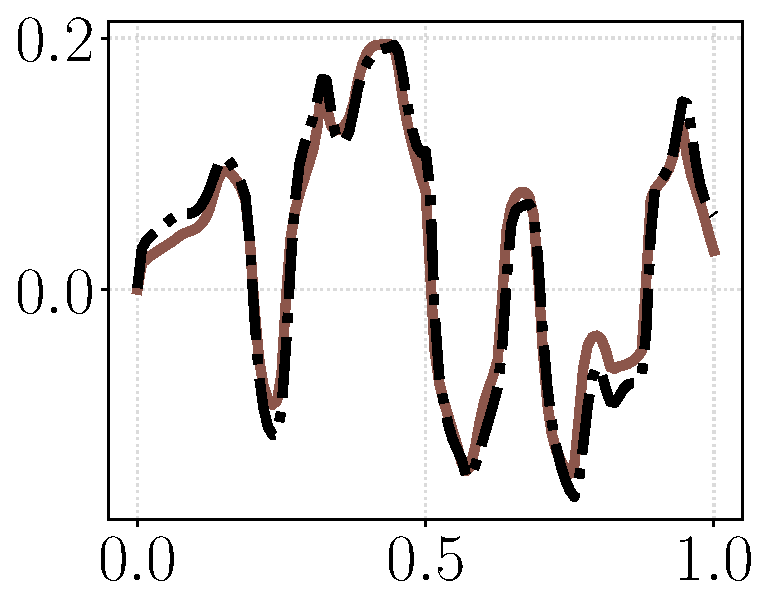
\includegraphics[width=0.245\linewidth]{figures/pk1_stress_23_median.pdf} \\
        & 31 & 32 & 33 \\
        &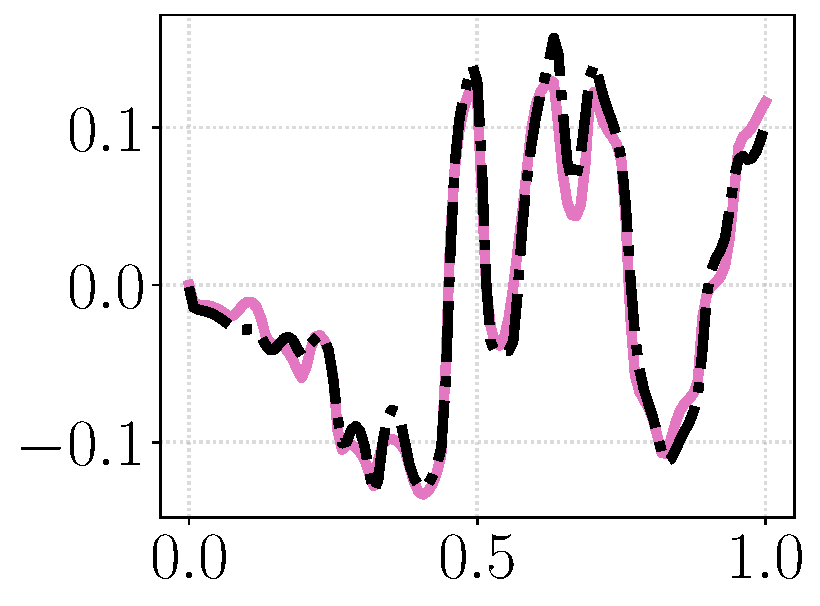
\includegraphics[width=0.26\linewidth]{figures/pk1_stress_31_median.pdf} &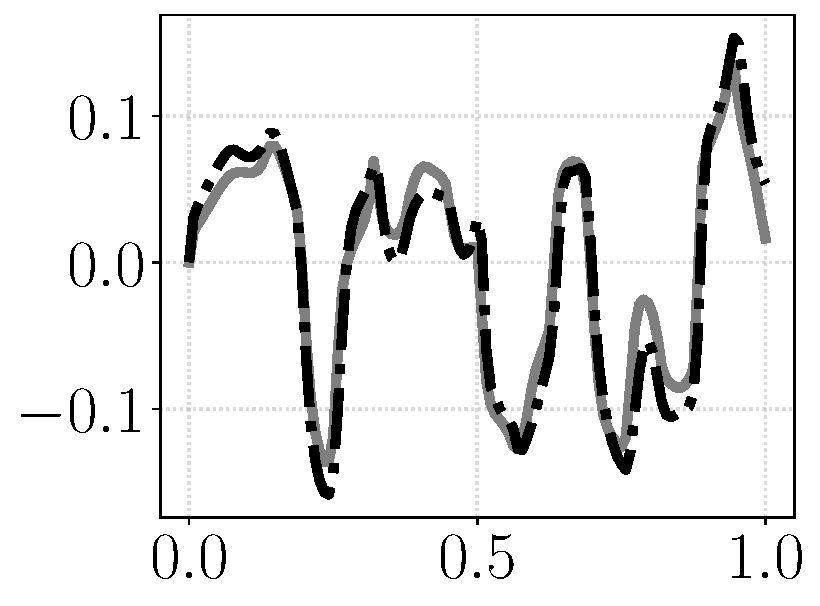
\includegraphics[width=0.26\linewidth]{figures/pk1_stress_32_median.pdf}  
         & 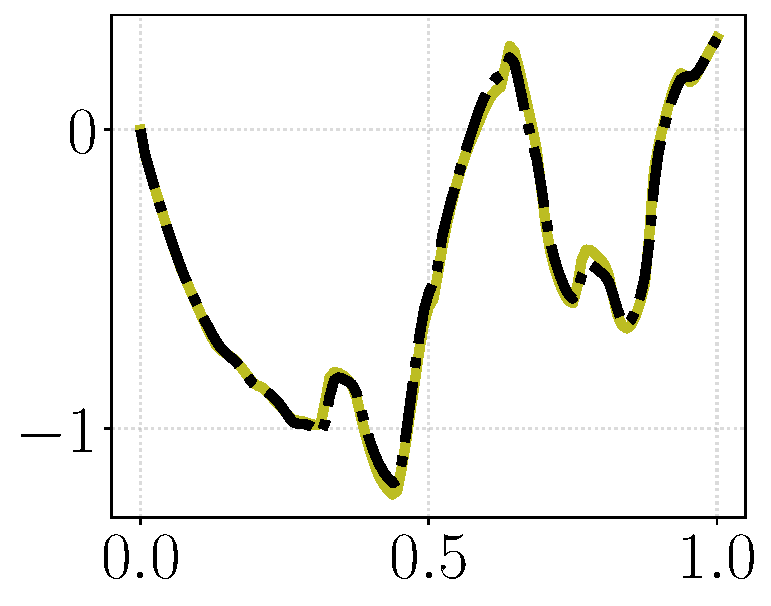
\includegraphics[width=0.245\linewidth]{figures/pk1_stress_33_median.pdf}\\
         & \multicolumn{3}{c}{Time (s)}
    \end{tabular}
    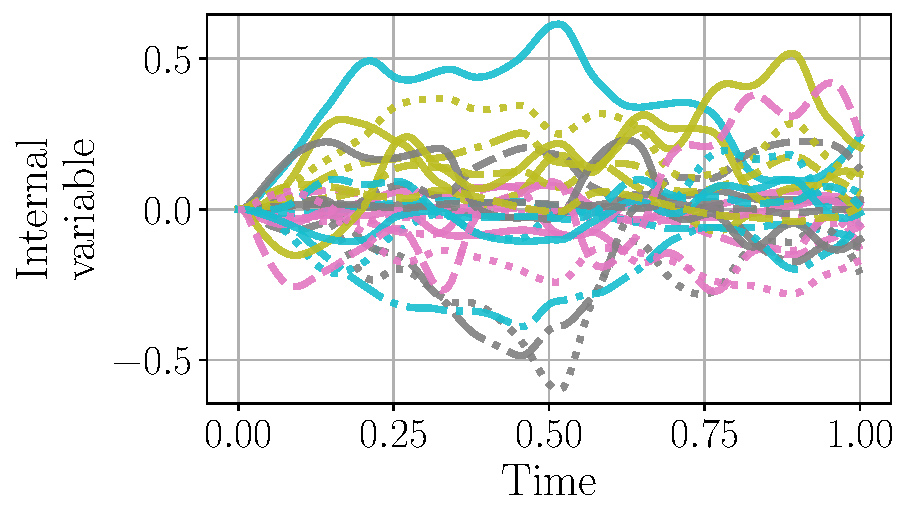
\includegraphics[width=0.6\linewidth]{figures/cp_internal_iv25_median.pdf}
    \addtolength{\tabcolsep}{5 pt}
    }
    
    \caption{(\emph{Top}) The test sample of the crystal plasticity dataset with a median relative stress prediction error (7.5\%) for the learned model. (\emph{Bottom left}) The stress-prediction components, where solid lines denote the reference homogenized response and dashed-dotted lines denote the stress response predicted by the learned model. (\emph{Bottom right}) The components of the internal variable predicted by the learned model.}
    \label{fig:cp_median_prediction}
\end{figure}
